% GIFT manuscript: AMIA structured draft. Use XeLaTeX for the two-page layout.
% Main text is on page 1; figures, tables, and references are on page 2.
% Values are transcribed from the original papers and the existing study reports.
% See evidence_notes.md for sources, metric definitions, and comparison limits.
\documentclass[10pt,letterpaper]{article}
\usepackage[margin=1in]{geometry}
\usepackage[T1]{fontenc}
\usepackage{newtxtext,newtxmath}
\usepackage{graphicx,booktabs,array,tabularx}
\usepackage[font=small,labelfont=bf,skip=4pt,hypcap=false]{caption}
\usepackage{xcolor}
\usepackage[hidelinks]{hyperref}
\usepackage{tikz}
\usetikzlibrary{arrows.meta,positioning}
\setlength{\parindent}{0pt}
\setlength{\parskip}{4pt}
\setlength{\textfloatsep}{7pt}
\setlength{\intextsep}{7pt}
\renewcommand{\arraystretch}{1.13}
\newcommand{\subhead}[1]{\par\vspace{3pt}\noindent\textbf{#1}\par\nobreak}
\newcolumntype{L}[1]{>{\raggedright\arraybackslash}p{#1}}
\hypersetup{pdftitle={GIFT: Glaucoma Imaging of Future Trajectories},pdfauthor={Sitar Eswar and Michael Gee}}

\definecolor{trainblue}{HTML}{176B9A}
\definecolor{traingreen}{HTML}{167865}
\definecolor{trainviolet}{HTML}{7750A5}
\definecolor{forecastorange}{HTML}{AC5A12}
\definecolor{forecastred}{HTML}{AC3C5C}
\newcommand{\fillin}[1]{\textcolor{forecastorange}{\textbf{[#1]}}}
\begin{document}
\begin{center}
{\fontsize{14}{16}\selectfont\bfseries GIFT: Glaucoma Imaging of Future Trajectories}\par
{\fontsize{12}{14}\selectfont\bfseries Sitar Eswar\textsuperscript{1}, Michael Gee, Doctor of Optometry\textsuperscript{2}}\par
{\fontsize{12}{14}\selectfont\bfseries \textsuperscript{1}Design Tech High School, Redwood City, California;\\
\textsuperscript{2}\fillin{Affiliation}, Foster City, California}
\end{center}
\vspace{-5pt}
\subhead{Abstract}
\emph{We developed GIFT (Glaucoma Imaging of Future Trajectories), an open-source research tool that generates future retinal images from one photograph at times up to five years ahead. In 1,636 test pairs from 49 patients, generated images achieved 0.9645 global similarity to processed real follow-up images. This supports single-photograph image generation for clinician assessment; demonstrating accurate glaucoma prediction and equivalence to multi-visit methods requires further evaluation.}

\subhead{Introduction}
Glaucoma damages the optic nerve, which carries visual information to the brain. Retinal photographs show its visible head, the optic disc, and central depression, the optic cup; changes in these structures help clinicians assess disease\textsuperscript{1}. We wanted to help clinicians see possible future changes before they occur. Earlier work predicts glaucoma from two visits\textsuperscript{2} or generates future images from several visits\textsuperscript{3}. We asked whether one photograph could provide useful forecasts for studying glaucoma onset and worsening, with less patient history.

\subhead{Methods}
We retrospectively studied Sequential Fundus Images for Glaucoma Forecast (SIGF)\textsuperscript{4}: 3,684 photographs from 405 eyes of 262 patients. We assigned each patient's images to one group, using 5,572 earlier--later pairs for training, 690 for choosing settings, and 1,636 for testing. PAPILA, a separate dataset, supplied expert disc and cup outlines for our measurement tool\textsuperscript{5}.

GIFT learns to generate images by removing added noise\textsuperscript{6}, guided by time and photographic vessel, nerve-fiber, and brightness patterns. Each forecast starts from the same real photograph. We measured image error and similarity against processed real follow-ups and an unchanged starting-image reference. Clinician assessment concerns resemblance and the amount of visible change.

\begin{center}
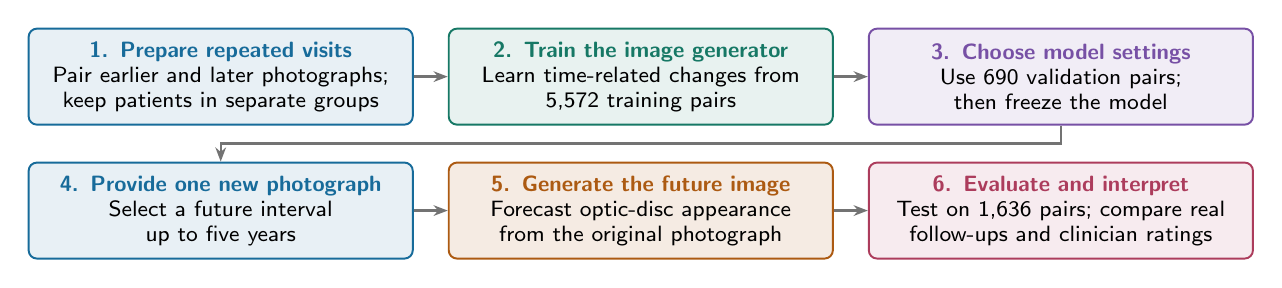
\begin{tikzpicture}[
 font=\sffamily\fontsize{8}{9}\selectfont,
 stage/.style={rounded corners=3pt,line width=0.7pt,text width=1.81in,
 minimum height=0.48in,align=center,inner sep=4pt},
 flow/.style={-{Stealth[length=1.8mm]},draw=black!55,line width=0.85pt}]
\node[stage,draw=trainblue,fill=trainblue!10] (a) {\textcolor{trainblue}{\textbf{1. Prepare repeated visits}}\\Pair earlier and later photographs;\\keep patients in separate groups};
\node[stage,draw=traingreen,fill=traingreen!10,right=0.17in of a] (b) {\textcolor{traingreen}{\textbf{2. Train the image generator}}\\Learn time-related changes from\\5,572 training pairs};
\node[stage,draw=trainviolet,fill=trainviolet!10,right=0.17in of b] (c) {\textcolor{trainviolet}{\textbf{3. Choose model settings}}\\Use 690 validation pairs;\\then freeze the model};
\node[stage,draw=trainblue,fill=trainblue!10,below=0.18in of a] (d) {\textcolor{trainblue}{\textbf{4. Provide one new photograph}}\\Select a future interval\\up to five years};
\node[stage,draw=forecastorange,fill=forecastorange!12,right=0.17in of d] (e) {\textcolor{forecastorange}{\textbf{5. Generate the future image}}\\Forecast optic-disc appearance\\from the original photograph};
\node[stage,draw=forecastred,fill=forecastred!10,right=0.17in of e] (f) {\textcolor{forecastred}{\textbf{6. Evaluate and interpret}}\\Test on 1,636 pairs; compare real\\follow-ups and clinician ratings};
\draw[flow] (a)--(b); \draw[flow] (b)--(c);
\draw[flow] (c.south)--++(0,-0.09in)-|(d.north);
\draw[flow] (d)--(e); \draw[flow] (e)--(f);
\end{tikzpicture}
\end{center}
\vspace{-5pt}

\subhead{Results}
Generated images closely resembled processed follow-ups: global similarity was 0.9645 (1 means identical), and average pixel error was 0.044255 on a 0--1 scale. The unchanged image gave nearly identical scores (Table~\ref{tab:heldout}); GIFT's error was slightly lower near three and five years. Two example eyes showed mean automatic cup-outline overlap of 0.869.

\textcolor{forecastorange}{\emph{Clinician-results template; complete after review:}} Dr. Gee reviewed \fillin{n} final follow-ups during \fillin{dates}. Mean similarity was \fillin{score}/5; \fillin{n/N; \%} showed about the same amount of change as the real image (Table~\ref{tab:review}).

\subhead{Discussion}
GIFT is an open-source research tool for clinicians to explore glaucoma-related appearance up to five years ahead from one photograph. Its contribution is the reduced input requirement; equal performance to multi-visit methods remains unproven. Image resemblance also needs validation against glaucoma onset and worsening. The approach could extend to other eye diseases with disease-specific longitudinal training and evaluation. Sitar Eswar led the model implementation and analysis.

\clearpage
\begin{table}[!ht]
\centering\small
\setlength{\tabcolsep}{4pt}
\begin{tabularx}{\textwidth}{@{}L{0.88in}L{1.03in}L{1.42in}>{\raggedright\arraybackslash}X@{}}
\toprule
\textbf{Study} & \textbf{Input history} & \textbf{What it produces} & \textbf{Generated versus real image evidence}\\
\midrule
Lin and colleagues [2] & 2 visits of the same eye & A future-glaucoma prediction & No generated images to compare.\\
Zhang and colleagues [3] & Several earlier visits of the same eye & A glaucoma prediction and a future retinal image & Two visual examples; no numerical image-similarity score reported.\\
GIFT (ours) & 1 image; future time & A future optic-disc image for clinician interpretation & Similarity: 0.9645. Pixel error: 0.044255. Tested on 1,636 image pairs.\\
\bottomrule
\end{tabularx}
\caption{Earlier approaches and GIFT. Zhang generates future images; Lin predicts glaucoma without image generation. Disease-classification scores cannot establish equal image quality across studies.}
\label{tab:literature}
\end{table}

\begin{table}[!ht]
\centering\small
\setlength{\tabcolsep}{3pt}
\begin{tabular}{@{}lrrrrrr@{}}
\toprule
\textbf{Time ahead} & \textbf{Pairs} & \textbf{GIFT error} & \shortstack{\textbf{Unchanged}\\\textbf{image error}} & \shortstack{\textbf{Error}\\\textbf{reduction}} & \shortstack{\textbf{GIFT}\\\textbf{similarity}} & \shortstack{\textbf{Unchanged}\\\textbf{image similarity}}\\
\midrule
All & 1,636 & 0.044255 & 0.044198 & $-0.13\%$ & 0.964467 & 0.964469\\
$\sim$1 year & 464 & 0.040055 & 0.039421 & $-1.61\%$ & 0.968325 & 0.968577\\
$\sim$3 years & 753 & 0.043956 & 0.044026 & $+0.16\%$ & 0.964745 & 0.964604\\
$\sim$5 years & 419 & 0.049445 & 0.049795 & $+0.70\%$ & 0.959694 & 0.959676\\
\bottomrule
\end{tabular}
\caption{Results from 49 test patients. Error is mean absolute error (lower is better); similarity is the global structural similarity index measure (1 is identical). Positive reduction favors GIFT. Scores use aligned, color-matched $128\times128$ targets with changes clipped to $\pm0.18$. Patient-averaged error difference: 0.000165; 95\% confidence interval from patient resampling: $[-0.000147,0.000513]$. Time groups: $\leq1.5$, $>1.5$--$3.5$, and $>3.5$--$5$ years.}
\label{tab:heldout}
\end{table}

\noindent\begin{minipage}[t]{0.36\textwidth}
\vspace{0pt}\centering
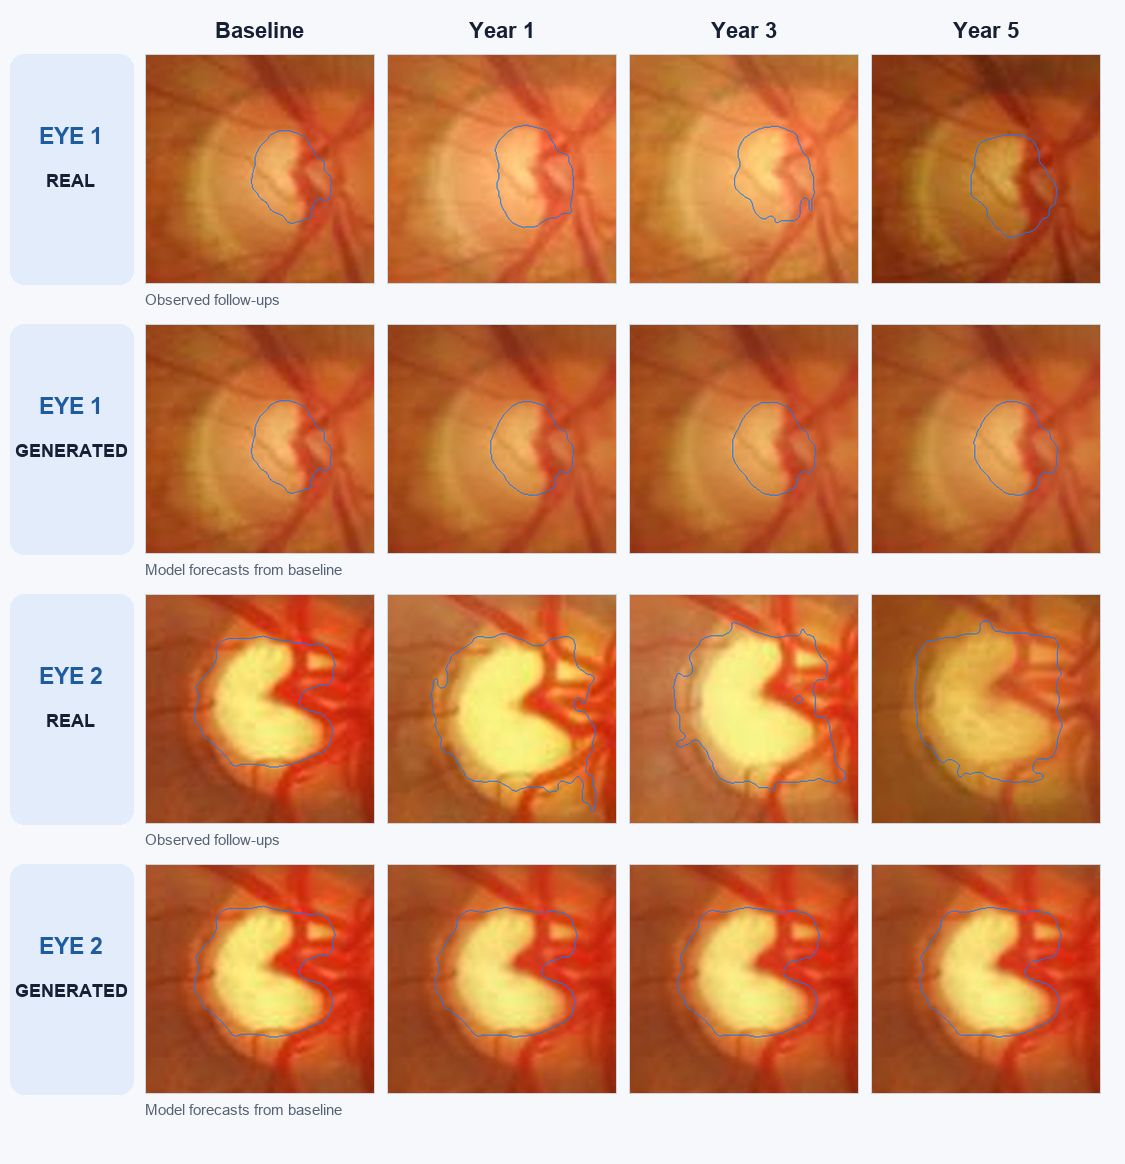
\includegraphics[width=0.94\linewidth]{figures/sigf_two_eyes_16_papila_contours.png}
\captionof{figure}{Two example eyes. Baseline is the starting photograph; generated is the forecast. Columns show visits nearest Years 1, 3, and 5. Blue lines mark automatic cup outlines.}
\label{fig:progression}
\end{minipage}\hfill
\begin{minipage}[t]{0.61\textwidth}
\vspace{0pt}\small\centering
\setlength{\tabcolsep}{4pt}
\begin{tabular}{@{}lrrr@{}}
\toprule
\textbf{Measure in example eyes} & \textbf{Year 1} & \textbf{Year 3} & \textbf{Year 5}\\
\midrule
Cup overlap (Dice score) & 0.860 & 0.869 & 0.879\\
Cup-to-disc height ratio error & 0.112 & 0.094 & 0.154\\
Vessel-pattern agreement & 0.456 & 0.589 & 0.369\\
Nerve-fiber pattern agreement & 0.641 & 0.765 & 0.616\\
\bottomrule
\end{tabular}
\captionof{table}{Automatic averages for the two example eyes. Dice measures cup-outline overlap; 1 is perfect. Height ratio divides cup height by disc height. Pattern agreement is correlation. These are photographic measures, not clinician ratings.}
\label{tab:examples}
\vspace{4pt}
\begin{tabularx}{\linewidth}{@{}Xr@{}}
\toprule
\textbf{Clinician-results template} & \textbf{Result}\\
\midrule
Final follow-ups reviewed (number) & \rule{0.55in}{0.3pt}\\
Mean similarity rating (1--5) & \rule{0.55in}{0.3pt}\\
About the same change (number/total; \%) & \rule{0.55in}{0.3pt}\\
Review dates & \rule{0.55in}{0.3pt}\\
\bottomrule
\end{tabularx}
\captionof{table}{Draft results skeleton. Similarity ranges from 1 (very different) to 5 (very similar). Use assessable cases as the denominator; report unable-to-assess counts separately. Complete blanks only after review.}
\label{tab:review}
\end{minipage}

\vspace{3pt}
{\centering\textbf{References}\par}\vspace{2pt}
\begingroup\footnotesize\raggedright\setlength{\parskip}{1pt}
1. European Glaucoma Society. Terminology and guidelines for glaucoma, 4th edition, part 1. Br J Ophthalmol. 2017;101:1--72. \href{https://doi.org/10.1136/bjophthalmol-2016-EGSguideline.001}{Article link}.

2. Lin M, Liu L, Gorden M, et al. Multi-scale multi-structure siamese network (MMSNet) for primary open-angle glaucoma prediction. In: Machine Learning in Medical Imaging. 2022;13583:436--445. \href{https://doi.org/10.1007/978-3-031-21014-3_45}{Article link}.

3. Zhang Y, Huang K, Yang X, et al. Coarse-to-fine latent diffusion model for glaucoma forecast on sequential fundus images. In: Medical Image Computing and Computer Assisted Intervention. 2024;15005:166--176. \href{https://doi.org/10.1007/978-3-031-72086-4_16}{Article link}.

4. Li L, Wang X, Xu M, Liu H, Chen X. DeepGF: glaucoma forecast using the sequential fundus images. In: Medical Image Computing and Computer Assisted Intervention. 2020;12265:626--635. \href{https://doi.org/10.1007/978-3-030-59722-1_60}{Article link}.

5. Kovalyk O, Morales-S\'{a}nchez J, Verd\'{u}-Monedero R, et al. PAPILA: dataset with fundus images and clinical data of both eyes of the same patient for glaucoma assessment. Sci Data. 2022;9:291. \href{https://doi.org/10.1038/s41597-022-01388-1}{Article link}.

6. Ho J, Jain A, Abbeel P. Denoising diffusion probabilistic models. Adv Neural Inf Process Syst. 2020;33:6840--6851. \href{https://proceedings.neurips.cc/paper/2020/hash/4c5bcfec8584af0d967f1ab10179ca4b-Abstract.html}{Paper link}.
\endgroup
\end{document}
